\documentclass[../thesis.tex]{subfiles}

\begin{document}
\vspace{-1\baselineskip}
Physics analysis inherently incurs uncertainties in the form of statistical and systematic uncertainties, depending on the source. Statistical uncertainties occur in this analysis from sample size of collected data and simulated \acs{MC} samples, and from the maximizing of the \acs{LH} function. Systematic uncertainties depend on identifiable sources in the analysis i.e. from detector and reconstruction effects (experimental uncertainties) or theoretical modeling (theoretical uncertainties). Systematic uncertainties are represented as nuisance parameters (\acs{NP}x) in the profile \acs{LH} fit. During the fit, systematic uncertainties with negligible impact on the final results can be pruned to simplify the statistical model and reduce computational complexity. This section outlines all uncertainties considered in this analysis.
%; in particular, experimental uncertainties are documented in \autoref{tab:syst_summary}, modeling uncertainties in \autoref{tab:syst_signal} and reducible background in \autoref{tab:syst_bg}.
%- Heavy pruning, 10\% on shape and normalization pruning \textcolor{red}{(to fit timeline?)}

\section{Experimental uncertainties}
\label{sec:sysexp}
%Instrumental \& minor

%\begin{table}[!htbp]
%  \centering
%  \scriptsize
%%  \setlength{\tabcolsep}{3pt} % Reduce column spacing
%%  \renewcommand{\arraystretch}{1.2} % Adjust row spacing
%  \caption{Summary of the experimental systematic uncertainties considered in this analysis.} 
%  \resizebox{0.8\textwidth}{!}{%
%%  \begin{threeparttable}
%  \label{tab:syst_summary}
%    \begin{tabular}{lc}
%      \toprule \midrule
%      Systematic uncertainty 			& Components	\\
%      \midrule
%      \multicolumn{2}{l}{\textbf{Event}} 		\\	\midrule
%      Luminosity 						& 1		\\
%      Pile-up reweighting				& 1		\\
%      \midrule
%      \multicolumn{2}{l}{\textbf{Electrons}}  	\\	\midrule
%      Trigger efficiency 				& 1 	\\
%%      Reconstruction efficiency\textsuperscript{\textdagger}						& 1 \\ 
%%      Identification efficiency\textsuperscript{\textdagger}						& 1 \\ 
%%      Isolation efficiency\textsuperscript{\textdagger} 							& 1 \\
%      Reconstruction efficiency			& 1 	\\ 
%      Identification efficiency			& 1 	\\ 
%      Isolation efficiency 				& 1 	\\
%      Energy scale       				& 1 	\\ 
%      Energy resolution  				& 1 	\\
%%      Charge identification (\acs{ECIDS}) efficiency\textsuperscript{\textdagger}	& 1 \\
%      Charge identification (\acs{ECIDS}) efficiency								& 1 \\
%      \midrule
%      \multicolumn{2}{l}{\textbf{Muons}}  		\\	\midrule
%      Trigger efficiency				& 2		\\
%      Track-to-vertex association efficiency										& 2 \\
%      Reconstruction/identification efficiency										& 2 \\
%      Low-\pT ($<15$ GeV) reconstruction/identification efficiency					& 2 \\
%      Isolation efficiency			 	& 2 	\\
%      Charge-independent momentum scale & 1 	\\
%      Charge-dependent momentum scale 	& 4 	\\ %GLOBAL/PTEXTRA?
%      Energy resolution (\acs{CB}) 		& 1 	\\
%      Energy resolution (ID \& MS) 		& 2 	\\
%      \midrule
%      \multicolumn{2}{l}{\textbf{Jets}}  		\\	\midrule
%      JES effective NP					& 15	\\
%      JES $\eta$ intercalibration		& 3  	\\
%      JES flavor composition 			& 2	 	\\
%      JES flavor response				& 1	 	\\
%      JES pile-up						& 4	 	\\
%      JES punch-through (FS/AF3)		& 2	 	\\
%      JES non-closure					& 1  	\\
%      JES high-\pT single particle		& 1	 	\\
%      JES $b$-jet response				& 1  	\\
%      \midrule
%      JER effective NP					& 12  	\\
%      JER data/MC (FS/AF3)				& 2  	\\
%%      \midrule
%      JVT efficiency					& 1  	\\
%      \midrule
%      GN2v01 $b$-tagging efficiency		& 85	\\
%      GN2v01 $c$-tagging efficiency		& 56 	\\
%      GN2v01 light-tagging efficiency	& 42 	\\
%    %   Jet PCBT high $p_T$ & $b$-tagging efficiency uncertainty on the extrapolation on high \pt-jets \\
%      %% no extrapolation uncertainties?
%      %% ATLAS\_FTAG\_GN2v01\_extrapolation &  $b$-tagging efficiency uncertainty on the extrapolation on high \pt-jets  \\ 
%      %% ATLAS\_FTAG\_GN2v01\_extrapolation\_from\_charm & $b$-tagging efficiency uncertainty on $\tau$-jets   \\
%      \midrule
%      \multicolumn{2}{l}{\textbf{\ETmiss track-based soft terms}}  \\	\midrule
%      Transversal resolution			& 1  	\\
%      Longitudinal resolution			& 1  	\\
%      Longitudinal energy scale			& 1  	\\
%      %	MET\_JetTrk\_Scale        & track MET scale uncertainty due to tracks in jets   \\
%      %	METTrigStat & \multirow{2}{*}{trigger efficiency uncertainty} -  \\
%      %	METTrigSyst & \\
%      \bottomrule
%    \end{tabular}
%%    \begin{tablenotes}
%%      \scriptsize
%%      \item \textsuperscript{\textdagger}Not ready for the analysis, but will be included
%%%      \item \textsuperscript{*}Not included
%%    \end{tablenotes}
%%  \end{threeparttable}
%}
%\end{table}

\subsection{Luminosity \& pile-up reweighting}
The uncertainty on the integrated luminosity of the 2015-2018 Run 2 data set is $0.83\%$ \citep{DAPR-2021-01}, obtained by the LUCID-2 detector \citep{LUCID2} for the primary luminosity measurements and complemented by the \acs{ID} and calorimeters. Pile-up was modeled in \acs{MC} and calibrated to data through pile-up reweighting, resulting in a set of calibration \acs{SF}s and associated uncertainties.

\subsection{Leptons}
In general, calibrating \acs{MC} simulations to match performance in data incurs uncertainties associated obtaining the MC-to-data calibration \acs{SF}s, which are in turn propagated to observables in the analysis. The data-to-\acs{MC} calibration of trigger, reconstruction, identification and isolation efficiencies for electrons and muons incur associated uncertainties, with separate systematic and statistical components for those related to muons. Similarly, electron energy scale, muon momentum scale and resolution are also subjected to calibration uncertainties estimated by re-simulating the events while varying the energy/momentum scale and resolution. Electron has an additional uncertainty related to \acs{ECIDS} efficiency. Muon has additional uncertainties for charge-independent and charge-dependent momentum scale, as well as detector-specific track resolution. Systematic uncertainties for electron reconstruction, identification, isolation, \acs{ECIDS} efficiencies and muon \acs{ID}/\acs{MS} energy resolution were not ready for the sample version used in this analysis, and are therefore not included.

\subsection{Jets}
Experimental uncertainties for jets are dominated by flavor tagging-related uncertainties, with subleading contributions from uncertainties related to \acs{JES} \citep{reco:jet_jes}, \acs{JER} \citep{reco:jet_jer} and \acs{JVT} \citep{syst:jvt_calib} calibrations. 

%\textcolor{red}{talk about JVT beforehand in ch4?}

\subsubsection*{Jet energy scale}
Uncertainties associated with \acs{JES} are determined using data from \acs{LHC} collisions along with \acs{MC} simulated samples \citep{reco:jet_jes}, decomposed into uncorrelated components:
\begin{itemize}
\item \textbf{Effective \acs{NP}s}: 15 total \pT-dependent uncertainty components measured in situ, grouped based on their origin (2 detector-related, 4 modeling-related, 3 mixed, 6 statistical-related)
\item \textbf{\acs{eta} intercalibration}: 6 total components (1 modeling-related, 4 non-closure and 1 statistical-related) associated with the correction of the forward jets' ($0.8\leq |\eta| < 4.5$) energy scale to that of the central jets ($|\eta| < 0.8$).
\item \textbf{Flavor composition \& response}: 2 components for relative quark-gluon flavor compositions in background and signal samples, and 2 components for responses to gluon-initiated versus quark-initiated jets.
\item \textbf{Pile-up subtraction}: 4 components, 2 for $\mu$ (\verb|OffsetMu|) and $N_\mathrm{PV}$ (\verb|OffsetNPV|) modeling, 1 for residual \pT-dependency (\verb|PtTerm|) and 1 for topology dependence on the per-event \pT density modeling (\verb|RhoTopology|).
\item \textbf{Punch-through effect treatment:} 2 terms for \acs{GSC} punch-through jet response deviation between data and \acs{MC}, one for each detector response simulation method (\acs{AF3} and \acs{FS}).
\item \textbf{Non-closure}: 1 term applied to \acs{AF3} sample to account for the difference between \acs{AF3} and \acs{FS} simulation.
\item \textbf{High-\pT single-particle response}: 1 term for the response to high-\pT jets from single-particle and test-beam measurements.
\item \textbf{$b$-jets response}: 1 term for the difference between $b$-jets and light-jets response.
\end{itemize}

\subsubsection*{Jet energy resolution}
Measurements of \acs{JER} were performed in bins of \pT and $\eta$, separately in data using in-situ techniques and in \acs{MC} simulation using dijet events \citep{reco:jet_jer}. This analysis uses the full correlation \acs{JER} uncertainty scheme provided for Run 2 analysis with 14 total components: 12 for effective \acs{NP}s and 2 for difference between data and \acs{MC}, separately for \acs{AF3} and \acs{FS} \citep{reco:jet_jer}.

\subsubsection*{Jet vertex tagging}
The uncertainty associated with \acs{JVT} is obtained by varying the \acs{JVT} efficiency \acs{SF}s within their uncertainty range \citep{syst:jvt_calib}. This uncertainty accounts for remaining contamination from pile-up jets after applying pile-up suppression and \acs{MC} generator choice.

\subsubsection*{Flavor tagging}
Calibration \acs{SF}s for $b$-tagging efficiencies and $c$-/light-jets mistagging rates are derived as a function of \pT for $b$-, $c$-, light-jets and \acs{PCBT} score. The full set of flavor tagging-related uncertainties was reduced in dimensions by diagonalizing the uncertainty covariance matrix via eigendecomposition \citep{ftag:calib}, resulting in a compact set of orthogonal \acs{NP}s for this analysis: 85 for $b$-jets, $56$ for $c$-jets and 42 for light-jets.

\subsection{Missing transverse energy}
Uncertainties on \acs{ETmiss} arise from possible mis-calibration of the soft-track component and are estimated using data-to-\acs{MC} comparison of the \pT scale and resolution between the hard and soft \acs{ETmiss} components \citep{reco:met}. These uncertainties are represented by three independent terms: 1 for scale uncertainty and 2 for resolution uncertainty of the parallel and perpendicular components.

%%%%%%%%%%%%%%%%%%%%%%%
%%% TABLE WITH NAME %%%
%%%%%%%%%%%%%%%%%%%%%%%

%\begin{table}[!ht]
%  \centering
%  \scriptsize
%  \begin{center}
%  \resizebox{\textwidth}{!}{%
%    \begin{tabular}{llcc}
%      \toprule \midrule
%      Systematic uncertainty	& Description	& Terms     & Scale [\%] \\
%      \midrule
%      \multicolumn{4}{c}{\textbf{Event}}  \\
%      \midrule
%      luminosity	& Luminosity 			& 1 & 0.83 \\
%      PRW\_DATASF	& Pile-up reweighting	& 1	& $\mathcal{O}(1) \sim \mathcal{O}(10)$\\
%      \midrule
%      \multicolumn{4}{c}{\textbf{Electrons}}  \\
%      \midrule
%      ATLAS\_EL\_SF\_TRIGGER	& Trigger efficiency & 1 & $\mathcal{O}(10^{-2}) \sim \mathcal{O}(10^{-1})$ \\
%      ATLAS\_EL\_SF\_RECO	& Reconstruction efficiency\textsuperscript{\textdagger} & 1 & $\mathcal{O}(10^{-1}) \sim \mathcal{O}(1)$  \\ 
%      ATLAS\_EL\_SF\_ID	& Identification efficiency\textsuperscript{\textdagger} & 1 & $\mathcal{O}(10^{-1}) \sim \mathcal{O}(1)$ \\ 
%      ATLAS\_EL\_SF\_ISO	& Isolation efficiency\textsuperscript{\textdagger} & 1 & $\mathcal{O}(10^{-1}) \sim \mathcal{O}(1)$ \\
%      EG\_SCALE\_ALL			& Energy scale       & 1 & $\mathcal{O}(10^{-2}) \sim \mathcal{O}(10^{-1})$ \\ 
%      EG\_RESOLUTION\_ALL		& Energy resolution  & 1 & $\mathcal{O}(10^{-2}) \sim \mathcal{O}(10^{-1})$ \\
%      ATLAS\_EL\_SF\_ChargeID\_Stat	& Charge identification (ECIDS) efficiency\textsuperscript{\textdagger} & 1	& $\mathcal{O}(10^{-1}) \sim \mathcal{O}(1)$ \\
%      \midrule
%      \multicolumn{4}{c}{\textbf{Muons}}  \\
%      \midrule
%      ATLAS\_MU\_SF\_TRIG\_Stat(Syst)	& Trigger efficiency						& 2 & $\mathcal{O}(10^{-1}) \sim \mathcal{O}(1)$\\
%      ATLAS\_MU\_SF\_TTVA\_Stat(Syst)	& Track-to-vertex association efficiency	& 2 & $\mathcal{O}(10^{-2}) \sim \mathcal{O}(10^{-1})$\\
%      ATLAS\_MU\_SF\_ID\_Stat(Syst)		& Reconstruction/identification efficiency	& 2 & $\mathcal{O}(10^{-1}) \sim \mathcal{O}(1)$\\
%      ATLAS\_MU\_SF\_ID\_Stat(Syst)\_LOWPT	& Low-\pT ($<15$ GeV) reconstruction/identification efficiency & 2 & $\mathcal{O}(10^{-1}) \sim \mathcal{O}(1)$\\
%      ATLAS\_MU\_SF\_ISO\_Stat(Syst)		& Isolation efficiency 				& 2 & $\mathcal{O}(10^{-1}) \sim \mathcal{O}(1)$\\ %syst
%      MUONS\_SCALE							& Charge-independent momentum scale & 1 & $\mathcal{O}(10^{-2}) \sim \mathcal{O}(10^{-1})$\\ 
%      MUONS\_SAGITTA						& Charge-dependent momentum scale 	& 4 & $\mathcal{O}(10^{-2}) \sim \mathcal{O}(10^{-1})$\\ %GLOBAL/PTEXTRA?
%      MUONS\_CB								& Energy resolution (CB) 			& 1 & $\mathcal{O}(10^{-2}) \sim \mathcal{O}(10^{-1})$\\ 
%%      Energy resolution (ID \& MS) & \\
%      \midrule
%      \multicolumn{4}{c}{\textbf{Jets}}  \\
%      \midrule
%      JES\_EffectiveNP						& JES effective NP				& 15 & $\mathcal{O}(10^{-2}) \sim \mathcal{O}(1)$\\
%      JES\_EtaIntercalibration				& JES $\eta$ intercalibration	& 3  & $\mathcal{O}(10^{-1}) \sim \mathcal{O}(1)$\\
%      JES\_Flavor\_Composition\_Bkg(Sig)	& JES flavor composition 		& 2	 & $\mathcal{O}(10^{-1}) \sim \mathcal{O}(1)$\\
%      JES\_Flavor\_Response					& JES flavor response			& 1	 & $\mathcal{O}(10^{-1}) \sim \mathcal{O}(1)$ \\
%      JES\_Pileup							& JES pile-up					& 4	 & $\mathcal{O}(10^{-1}) \sim \mathcal{O}(10)$ \\
%      JES\_PunchThrough\_MC16				& JES punch-through (FS/AF3\textsuperscript{*})		& 2	 & $<\mathcal{O}(10^{-2})$ \\
%      JES\_RelativeNonClosure\_MC20(AF3)	& JES non-closure				& 1  & $\mathcal{O}(10^{-2}) \sim \mathcal{O}(10^{-1})$ \\
%      JES\_SingleParticle\_HightPt			& JES high-\pT single particle	& 1	 & $<\mathcal{O}(10^{-2})$  \\
%      BJETS\_Response						& JES $b$-jet response			& 1  & $\mathcal{O}(10^{-1}) \sim \mathcal{O}(1)$ \\
%      \midrule
%      JER\_EffectiveNP\_[1-12]				& JER effective NP				& 12  & $\mathcal{O}(10^{-1}) \sim \mathcal{O}(1)$ \\
%      JER\_DataVsMC\_MC16					& JER data/MC (FS/AF3\textsuperscript{*})		& 2  & $\mathcal{O}(10^{-1}) \sim \mathcal{O}(1)$ \\
%      \midrule
%      NNJvtEfficiency						& JVT efficiency				& 1  & $\mathcal{O}(10^{-1}) \sim \mathcal{O}(1)$ \\
%      \midrule
%      FT\_EFF\_Eigen\_B\_[0-84]		& GN2v01 $b$-tagging efficiency ($b$-jets)	& 85 & $\mathcal{O}(10^{-2}) \sim \mathcal{O}(1)$ \\ %45?
%      FT\_EFF\_Eigen\_C\_[0-55]		& GN2v01 $b$-tagging efficiency ($c$-jets)	& 56 & $\mathcal{O}(10^{-2}) \sim \mathcal{O}(1)$ \\ %20?
%      FT\_EFF\_Eigen\_Light\_[0-41]	& GN2v01 $b$-tagging efficiency (light-jets)	& 42 & $\mathcal{O}(10^{-2}) \sim \mathcal{O}(1)$ \\ %20?
%    %   Jet PCBT high $p_T$ & $b$-tagging efficiency uncertainty on the extrapolation on high \pt-jets \\
%      %% no extrapolation uncertainties?
%      %% ATLAS\_FTAG\_GN2v01\_extrapolation &  $b$-tagging efficiency uncertainty on the extrapolation on high \pt-jets  \\ 
%      %% ATLAS\_FTAG\_GN2v01\_extrapolation\_from\_charm & $b$-tagging efficiency uncertainty on $\tau$-jets   \\
%      \midrule
%      \multicolumn{4}{c}{\textbf{\ETmiss-Terms}}  \\
%      \midrule
%      MET\_SoftTrk\_ResoPerp	& Track-based soft term for transversal resolution	& 1  & $\mathcal{O}(10^{-2}) \sim \mathcal{O}(10^{-1})$  \\
%      MET\_SoftTrk\_ResoPara	& Track-based soft term for longitudinal resolution	& 1  & $\mathcal{O}(10^{-2}) \sim \mathcal{O}(10^{-1})$  \\
%      MET\_SoftTrk\_Scale		& Track-based soft term for longitudinal scale		& 1  & $\mathcal{O}(10^{-2}) \sim \mathcal{O}(10^{-1})$  \\
%      %	MET\_JetTrk\_Scale        & track MET scale uncertainty due to tracks in jets   \\
%      %	METTrigStat & \multirow{2}{*}{trigger efficiency uncertainty} -  \\
%      %	METTrigSyst & \\
%      \bottomrule
%    \end{tabular}}
%  \end{center}
%  \caption{Summary of the experimental systematic uncertainties considered in this analysis.} 
%  \label{tab:syst_summary}
%\end{table}

%%%%%%%%%%%%%%%%%%%%%%%%
%%% TABLE WITH SCALE %%%
%%%%%%%%%%%%%%%%%%%%%%%%

%\begin{table}[!htbp]
%  \centering
%  \scriptsize
%  \caption{Summary of the experimental systematic uncertainties considered in this analysis.} 
%  \label{tab:syst_summary}
%  \begin{center}
%  \resizebox{\textwidth}{!}{%
%    \begin{tabular}{lcc}
%      \toprule \midrule
%      Systematic uncertainty & Terms     & Scale [\%] \\
%      \midrule
%      \multicolumn{3}{c}{\textbf{Event}}  \\
%      \midrule
%      Luminosity 			& 1 & 0.83 \\
%      Pile-up reweighting	& 1	& $\mathcal{O}(1) \sim \mathcal{O}(10)$\\
%      \midrule
%      \multicolumn{3}{c}{\textbf{Electrons}}  \\
%      \midrule
%      Trigger efficiency & 1 & $\mathcal{O}(10^{-2}) \sim \mathcal{O}(10^{-1})$ \\
%      Reconstruction efficiency\textsuperscript{\textdagger} & 1 & $\mathcal{O}(10^{-1}) \sim \mathcal{O}(1)$  \\ 
%      Identification efficiency\textsuperscript{\textdagger} & 1 & $\mathcal{O}(10^{-1}) \sim \mathcal{O}(1)$ \\ 
%      Isolation efficiency\textsuperscript{\textdagger} & 1 & $\mathcal{O}(10^{-1}) \sim \mathcal{O}(1)$ \\
%      Energy scale       & 1 & $\mathcal{O}(10^{-2}) \sim \mathcal{O}(10^{-1})$ \\ 
%      Energy resolution  & 1 & $\mathcal{O}(10^{-2}) \sim \mathcal{O}(10^{-1})$ \\
%      Charge identification (ECIDS) efficiency\textsuperscript{\textdagger} & 1	& $\mathcal{O}(10^{-1}) \sim \mathcal{O}(1)$ \\
%      \midrule
%      \multicolumn{3}{c}{\textbf{Muons}}  \\
%      \midrule
%      Trigger efficiency (stat/sys)				& 2 & $\mathcal{O}(10^{-1}) \sim \mathcal{O}(1)$\\
%      Track-to-vertex association efficiency (stat/sys)	& 2 & $\mathcal{O}(10^{-2}) \sim \mathcal{O}(10^{-1})$\\
%      Reconstruction/identification efficiency (stat/sys)	& 2 & $\mathcal{O}(10^{-1}) \sim \mathcal{O}(1)$\\
%      Low-\pT ($<15$ GeV) reconstruction/identification efficiency (stat/sys) & 2 & $\mathcal{O}(10^{-1}) \sim \mathcal{O}(1)$\\
%      Isolation efficiency (stat/sys) 				& 2 & $\mathcal{O}(10^{-1}) \sim \mathcal{O}(1)$\\ %syst
%      Charge-independent momentum scale & 1 & $\mathcal{O}(10^{-2}) \sim \mathcal{O}(10^{-1})$\\ 
%      Charge-dependent momentum scale 	& 4 & $\mathcal{O}(10^{-2}) \sim \mathcal{O}(10^{-1})$\\ %GLOBAL/PTEXTRA?
%      Energy resolution (CB) 			& 1 & $\mathcal{O}(10^{-2}) \sim \mathcal{O}(10^{-1})$\\ 
%      Energy resolution (ID \& MS)\textsuperscript{*} & 2 & $\mathcal{O}(10^{-2}) \sim \mathcal{O}(10^{-1})$\\ 
%%      Energy resolution (ID \& MS) & \\
%      \midrule
%      \multicolumn{3}{c}{\textbf{Jets}}  \\
%      \midrule
%      JES effective NP				& 15 & $\mathcal{O}(10^{-2}) \sim \mathcal{O}(1)$\\
%      JES $\eta$ intercalibration	& 3  & $\mathcal{O}(10^{-1}) \sim \mathcal{O}(1)$\\
%      JES flavor composition 		& 2	 & $\mathcal{O}(10^{-1}) \sim \mathcal{O}(1)$\\
%      JES flavor response			& 1	 & $\mathcal{O}(10^{-1}) \sim \mathcal{O}(1)$ \\
%      JES pile-up					& 4	 & $\mathcal{O}(10^{-1}) \sim \mathcal{O}(10)$ \\
%      JES punch-through (FS/AF3)		& 2	 & $<\mathcal{O}(10^{-2})$ \\
%      JES non-closure				& 1  & $\mathcal{O}(10^{-2}) \sim \mathcal{O}(10^{-1})$ \\
%      JES high-\pT single particle	& 1	 & $<\mathcal{O}(10^{-2})$  \\
%      JES $b$-jet response			& 1  & $\mathcal{O}(10^{-1}) \sim \mathcal{O}(1)$ \\
%      \midrule
%      JER effective NP				& 12  & $\mathcal{O}(10^{-1}) \sim \mathcal{O}(1)$ \\
%      JER data/MC (FS/AF3)		& 2  & $\mathcal{O}(10^{-1}) \sim \mathcal{O}(1)$ \\
%      \midrule
%      JVT efficiency				& 1  & $\mathcal{O}(10^{-1}) \sim \mathcal{O}(1)$ \\
%      \midrule
%      GN2v01 $b$-tagging efficiency ($b$-jets)	& 85 & $\mathcal{O}(10^{-2}) \sim \mathcal{O}(1)$ \\ %45?
%      GN2v01 $b$-tagging efficiency ($c$-jets)	& 56 & $\mathcal{O}(10^{-2}) \sim \mathcal{O}(1)$ \\ %20?
%      GN2v01 $b$-tagging efficiency (light-jets)	& 42 & $\mathcal{O}(10^{-2}) \sim \mathcal{O}(1)$ \\ %20?
%    %   Jet PCBT high $p_T$ & $b$-tagging efficiency uncertainty on the extrapolation on high \pt-jets \\
%      %% no extrapolation uncertainties?
%      %% ATLAS\_FTAG\_GN2v01\_extrapolation &  $b$-tagging efficiency uncertainty on the extrapolation on high \pt-jets  \\ 
%      %% ATLAS\_FTAG\_GN2v01\_extrapolation\_from\_charm & $b$-tagging efficiency uncertainty on $\tau$-jets   \\
%      \midrule
%      \multicolumn{3}{c}{\textbf{\ETmiss}}  \\
%      \midrule
%      Track-based soft term for transversal resolution	& 1  & $\mathcal{O}(10^{-2}) \sim \mathcal{O}(10^{-1})$  \\
%      Track-based soft term for longitudinal resolution	& 1  & $\mathcal{O}(10^{-2}) \sim \mathcal{O}(10^{-1})$  \\
%      Track-based soft term for longitudinal scale		& 1  & $\mathcal{O}(10^{-2}) \sim \mathcal{O}(10^{-1})$  \\
%      %	MET\_JetTrk\_Scale        & track MET scale uncertainty due to tracks in jets   \\
%      %	METTrigStat & \multirow{2}{*}{trigger efficiency uncertainty} -  \\
%      %	METTrigSyst & \\
%      \bottomrule
%    \end{tabular}}
%  \end{center}
%\end{table}

\section{Modeling uncertainties}
\label{sec:syst_mod}
\subsection{Signal and irreducible background uncertainties}
The signal and background samples used are modeled using \acs{MC} simulation. Most uncertainties on simulation parameters (e.g. generator choice, \acs{PS} model) are estimated by varying the relevant parameters and comparing them with the nominal sample. Uncertainties involving \acs{PDF} in particular for most processes in the analysis are set to a flat 1\% uncertainty. Cross-section uncertainties were considered for all irreducible background except \ttW, which is normalized in dedicated \acs{CR}s following section \ref{sec:ttW_BG}. 
Extra uncertainties for the production of four or more $b$-jets (additional $b$-jets) in association with $t\bar{t}X$ and \acs{HF} jets were also considered due to a lack of theoretical predictions or dedicated measurements, rendering \acs{MC} modeling challenging. Uncertainties from missing higher-order \acs{QCD} corrections in \acs{MC} simulation are estimated by varying the renormalization scale $\mu_R$ and factorization scale $\mu_F$ within seven different combinations
\[
(\mu_R, \mu_F) = \{(0.5,0.5), (0.5,1), (1,0.5), (1,1), (1,2), (2,1), (2,2)\}.
\]
%- pdf uncertainty: flat 1\% for \ttZp, \tttt, \ttZ, \ttH, envelope of differences between nominal vs. other pdf choices for \ttt
Process-specific uncertainty treatments are detailed below.

\subsubsection*{SM \tttt background}
The generator uncertainty for the \acs{SM} \tttt background was evaluated between a nominal sample of \mgamc and \sherpa. The parton shower uncertainty was evaluated between \pythia and \herwig. The cross-section uncertainty was estimated to be 20\% computed from a prediction at \acs{NLO} in \acs{QCD}+\acs{EW} \citep{Frederix:2017wme}.

\subsubsection*{\ttt background}
The cross-section uncertainty for \ttt was estimated to be 30\% computed from a prediction at \acs{NLO} in \acs{QCD}+\acs{EW} \citep{Frederix:2017wme}. Events with additional $b$-jets also incur a 50\% uncertainty.

\subsubsection*{\ttW, \ttZ, \ttH backgrounds}
For \ttW, \ttZ and \ttH backgrounds, an uncertainty of 50\% is assigned to events with one additional truth $b$-jets that did not originate from a top quark decay, and an added 50\% uncertainty is assigned to events with two or more \citep{TOPQ-2017-12} additional $b$-jets. The generator uncertainty was estimated for \ttZ using a \mgamc nominal sample and a \sherpa sample, and for \ttH using \textsc{PowhegBox} samples interfaced with \pythia (nominal) and \textsc{Herwig7}. Cross-section uncertainties of 12\% and 10\% were applied to \ttZ and \ttH respectively \citep{deFlorian:2016spz}. No \ttW cross-section or \acs{PDF} uncertainty was considered since the normalizations and jet multiplicity spectrum for \ttW are estimated using the data-driven method described in section \ref{sec:ttW_BG}.

\subsubsection*{Other backgrounds}
Other backgrounds include processes with small overall contribution in the \acs{SR}. The cross-section uncertainty for $tZ$ and $tWH$ is considered to be 30\% \citep{ATLAS-CONF-2017-052,Demartin_2017}. A conservative cross-section uncertainty of 50\% is applied to \ttVV, $VVV$ and $VH$. For $VV$, the cross-section uncertainty is dependent on jet multiplicity and is considered to be 20\%/50\%/60\% for events with $\leq 3$/$4$/$\geq 5$ jets \citep{STDM-2018-03}. For $VV$, \ttVV, $VVV$ and $VH$ events with additional truth $b$-jets, an uncertainty of 50\% is applied.

%\begin{table}[!htbp]
%  \centering
%  \scriptsize
%  \caption{\label{tab:syst_signal}Summary of signal and irreducible background modeling uncertainties considered in this analysis. Scale refers to the approximate effect of the uncertainty within the inclusive \acs{SR}.
%\textcolor{red}{(fit with inclusive SR to find scale. Also check no. of components.)}}
%  \begin{center}
%  \resizebox{0.72\textwidth}{!}{%
%  \begin{threeparttable}
%    \begin{tabular}{lcr}
%      \toprule\midrule
%      Systematic uncertainty					& Component		& Scale\textsuperscript{\textdagger} 	\\
%      \midrule
%      \multicolumn{3}{l}{\textbf{BSM \ttZp modeling}}						\\	\midrule
%      Renormalization \& factorization scale	& 1				&			\\
%      PDF										& 1				& 1\%		\\
%      \midrule
%      \multicolumn{3}{l}{\textbf{SM \tttt modeling}}						\\	\midrule
%      Cross-section 							& 1				& 20\%		\\
%      Renormalization \& factorization scale 	& 1				&			\\
%      PDF 										& 1				& 1\%		\\
%      Generator choice 							& 1				&			\\
%      Parton shower model 						& 1				&			\\
%      %Higher-order EW corrections
%      \midrule
%      \multicolumn{3}{l}{\textbf{\ttt modeling}}  							\\	\midrule
%      Cross-section 							& 1				& 30\%		\\
%      Renormalization \& factorization scale 	& 1				&			\\
%%     PDF 										& 1				& 1\%		\\
%      Additional $b$-jets 						& 2				& 50\%		\\
%      \midrule
%      \multicolumn{3}{l}{\textbf{\ttW modeling}}  							\\	\midrule
%      Renormalization \& factorization scale 	& 1				&			\\
%      Generator choice 							& 1				&			\\
%      Additional $b$-jets 						& 2				& 50-100\%	\\
%      \midrule
%      \multicolumn{3}{l}{\textbf{\ttZ modeling}}  							\\	\midrule
%      Cross-section 							& 1				& 10\%		\\
%      Renormalization \& factorization scale 	& 1				&			\\
%      PDF 										& 1				& 1\%		\\
%      Generator choice 							& 1				&			\\
%      Additional $b$-jets 						& 2				& 50-100\%	\\
%      \midrule
%      \multicolumn{3}{l}{\textbf{\ttH modeling}}  							\\ 	\midrule
%      Cross-section 							& 1				& 12\%		\\
%      Renormalization \& factorization scale 	& 1				&			\\
%      PDF 										& 1				& 1\%		\\
%      Generator choice 							& 1				&			\\
%      Additional $b$-jets 						& 2				& 50-100\%	\\
%      \midrule
%      \multicolumn{3}{l}{\textbf{Other background modeling}}  				\\	\midrule
%      Cross-section 							& 6				& 30-60\%	\\
%      Additional $b$-jets 						& 3				& 50\%		\\
%      \bottomrule
%    \end{tabular}
%    \begin{tablenotes}
%      \scriptsize
%      \item \textsuperscript{\textdagger}approximate, varies during fitting
%%      \item \textsuperscript{*}Not included
%    \end{tablenotes}
%  \end{threeparttable}
%  }
%  \end{center}
%\end{table}

\subsection{Reducible background uncertainties}
Reducible backgrounds consist of $t\bar{t}$/$V$+\acs{HF} jets and single top events. Reducible background has small contamination within the \acs{SR}, thus uncertainties related to reducible background have minor impact. Treatment for reducible background in this analysis largely follows Ref. \citep{tttt_obs}, except for \acs{QmisID}.

\subsubsection*{Charge misidentification}
Uncertainties on the \acs{QmisID} background originate from the charge flip rates obtained using the data-driven method described in section \ref{sec:qmisid}. Four sources of uncertainty were considered: statistical uncertainty from the maximum \acs{LLH} estimation using \autoref{eq:qmisid_llh}; uncertainty from choice of the $Z$-mass window and sidebands; non-closure uncertainty defined as the relative difference between the number of \acs{SS} and \acs{OS} events; and statistical uncertainty from the $N_\text{jets}$ dependency correction \acs{SF}s. The combined uncertainties from all four sources are calculated separately for each region involved in section \ref{sec:qmisid}, and are treated as correlated across all regions. \autoref{fig:syst:qmisid} shows the uncertainty calculated for \acs{SR}.

\begin{figure}[!htb]
\begin{center}
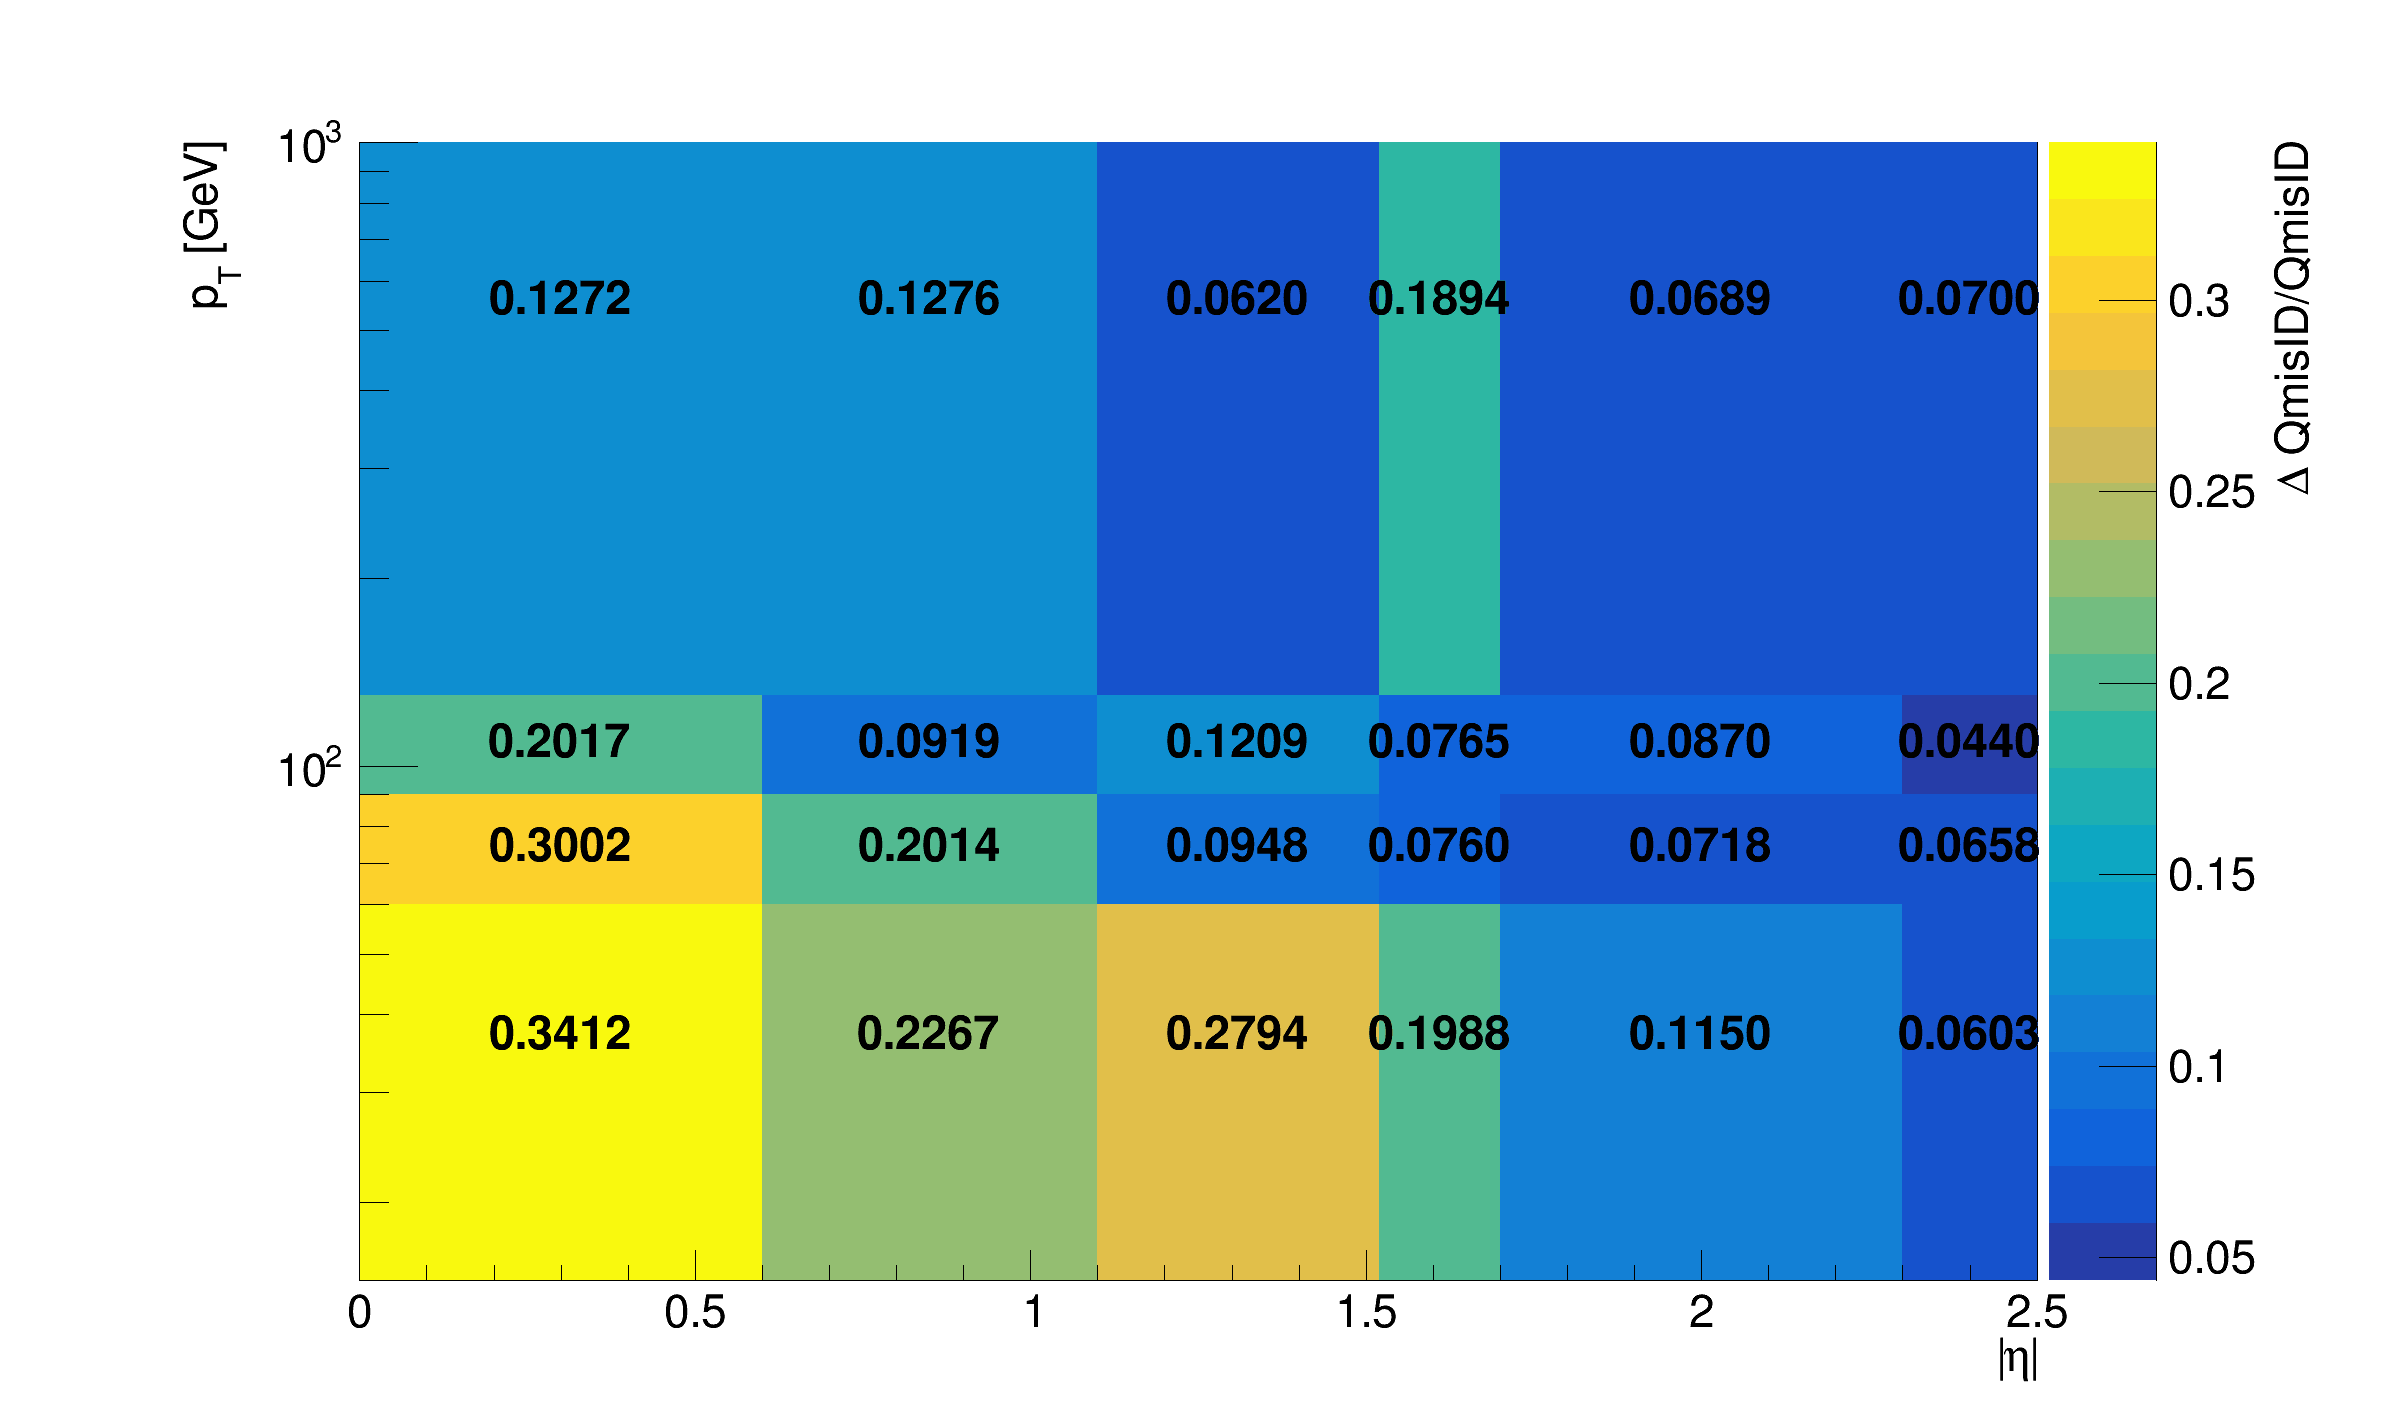
\includegraphics[width=0.9\linewidth]{fig/syst_qmisid_combined.png}
\caption{\label{fig:syst:qmisid}Combined \acs{QmisID} uncertainty rate for \acs{SR} in bins of $|\eta|$ and \pT.}
\end{center}
\end{figure}

%These uncertainties originate from uncertainties on electron charge flip rates. The uncertainty is determined independently in the conversion and \ttW control regions and treated as correlated among all regions.

\subsubsection*{Internal (low $\gamma^{*}$) and material conversion}
The normalization for internal and material conversion backgrounds are free parameters in the fit, as a result the only uncertainties evaluated are from the shape of the distributions used in the template fit method (see section \ref{sec:template}). The uncertainties on internal (material) conversion are estimated based on the difference between data and \acs{MC} prediction in a region enriched in $Z+\gamma \rightarrow \mu^+\mu^- + e^+e^-$ events.
%internal/material - 21%/33%

\subsubsection*{Heavy-flavor non-prompt lepton}
Similar to the conversion backgrounds, the uncertainties on non-prompt \acs{HF} decays come from the shape of the distributions, and are estimated by comparing data and \acs{MC} prediction between all regions in the analysis on a per bin basis. The events used are required to contain at least one \textit{Loose} reconstructed lepton used in the region selection criteria detailed in \autoref{tab:ana_regions} to maintain orthogonality with the \acs{SR}.
% ranging from 20-100\% across bins and SRs 

\subsubsection*{Light-flavor decays and other fake/non-prompt backgrounds}
A conservative normalization uncertainty of 100\% is assigned for light-flavor non-prompt lepton background \citep{bg:ttH_ttW_ML}, and an ad-hoc normalization uncertainty of 30\% is applied to all other fake and non-prompt backgrounds. The shape uncertainties for these backgrounds are negligible.




%\begin{table}[!htb]
%  \caption{\label{tab:syst_bg}Caption}
%  \scriptsize
%  \begin{center}
%  \resizebox{0.6\textwidth}{!}{%
%    \begin{tabular}{lcr}
%      \toprule \midrule
%      Systematic uncertainty	& Terms     & Scale	\\
%      \midrule
%      \multicolumn{3}{l}{\textbf{Reducible SM background}}  \\
%      \midrule
%      $t\bar{t}/V/t$+jets & 2 & 30\% \\
%      Charge misidentification & 1 & \\
%      \midrule
%      \multicolumn{3}{l}{\textbf{Fake \& non-prompt background}}  \\
%      \midrule
%      Low $\gamma^{*}$ & 1 & 21\%	\\
%      Material conversion & 1 & 30\% \\
%      HF $e$ & 1 & \\
%      HF $\mu$ & 1 & \\
%      Light-flavor decays & 1 & 100\% \\
%      Other fakes & 1 & 30\% \\
%      \bottomrule
%    \end{tabular}}
%  \end{center}
%\end{table}


\end{document}